\documentclass[10pt,a4paper]{article}
\usepackage[a4paper, total={6.5in, 9in}]{geometry}
\usepackage[latin1]{inputenc}
\usepackage{amsmath}
\usepackage{amsfonts}
\usepackage{amssymb}
\usepackage{mathtools}
\usepackage{graphicx}
\usepackage{float}
\usepackage[usenames, dvipsnames]{color}
\usepackage{fancyhdr}
\usepackage{enumitem}
\usepackage{listings}
\setlength{\headheight}{15.2pt}
\pagestyle{fancy}
\setlength{\parindent}{0em}
\setlength{\parskip}{10pt}
\setlist[enumerate,1]{label=\alph*)}
\setlist[enumerate,2]{label=(\roman*)}
\definecolor{LGray}{gray}{0.9}
\definecolor{deepgreen}{rgb}{0,0.5,0}
\lstset{language=python, tabsize=4, breaklines=true, postbreak=\mbox{\textcolor{red}{$\hookrightarrow$}\space}, basicstyle=\linespread{0.7}\ttfamily, commentstyle=\color{deepgreen},} 
\newcommand*\diff{\mathop{}\!\mathrm{d}}



\begin{document}
\title{COMP90086 Assignment 2}
\author{Benjamin Cheng-Hsien Yi}
\rhead{Benjamin Cheng-Hsien Yi - 1152795}
\lhead{COMP90086 Assignment 2}
	
\section{CNN implementation}
\subsection{Basic architecture}
Training accuracy increases over epochs, resulting in 83\% accuracy after 20 epochs of fitting. Validation accuracy also increases, but at a lower rate, leading to 65\% accuracy after 20 epochs of fitting. This is indicative of overfitting on the training set, as the training accuracy is higher than the validation accuracy. This divergence, which increases the more fitting is done (also indicative of overfitting), can be seen in figure \ref{fig:11}.

\begin{figure}[H]
	\centering
	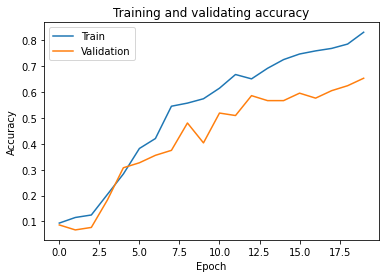
\includegraphics[width=0.7\linewidth]{images/11}
	\caption{Divergence of training and validation accuracies on basic CNN}
	\label{fig:11}
\end{figure}

\newpage
\subsection{Regularisation and data augmentation}
Regularisation was added via dropout after convolution layers, with a rate of 10\%. Data augmentation was performed by adding new layers to horizontally flip, rotate, and zoom each training image with a value of 10\% for both rotation and zoom. These values were chosen after ad-hoc non-exhaustive grid-search, for which the results can be seen in table \ref{Tab:ra}.

\begin{table}[H]
\centering
\begin{tabular}{|c|c|c|c|c|}
	\hline
	Dropout rate & Rotation value & Zoom value & Training accuracy & Validation accuracy \\
	\hline
	0.1 & 0.1 & 0.1 & 51\% & 52\% \\
	\hline
	0.2 & 0.1 & 0.1 & 52\% & 48\% \\
	\hline
	0.3 & 0.1 & 0.1 & 43\% & 47\% \\
	\hline
	0.1 & 0.2 & 0.1 & 33\% & 31\% \\
	\hline
	0.1 & 0.3 & 0.1 & 20\% & 15\% \\
	\hline
	0.1 & 0.1 & 0.2 & 50\% & 52\% \\
	\hline
	0.1 & 0.1 & 0.3 & 46\% & 50\% \\
	\hline
\end{tabular}
\caption{Parameter tuning results for CNN}
\label{Tab:ra}
\end{table}

While both training accuracy and validation accuracy has dropped in the new CNN from 83\% to 51\% and 65\% to 52\% respectively, the difference between training and validation accuracies has disappeared. This suggests overfitting is less present in the new model. This can be seen in figure \ref{fig:12} by how closely the training and validation accuracies track each other through the epochs. Note the difference to figure \ref{fig:11} where without these steps, the accuracies diverge. The overall decrease in validation accuracy is likely explained by the increase in sample size due to the data augmentation layer.

\begin{figure}[H]
	\centering
	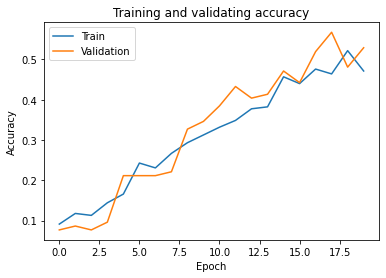
\includegraphics[width=0.7\linewidth]{images/12}
	\caption{Divergence of training and validation accuracies on new CNN}
	\label{fig:12}
\end{figure}

\newpage
\section{Error analysis}
The overall classification accuracy of the CNN on the test set was 54\%.
The individual accuracies for each class is presented in table \ref{Tab:class_acc}.

\begin{table}[H]
	\centering
	\begin{tabular}{|c|c|}
		\hline
		Class & Accuracy \\
		\hline
		bridge & 29\% \\
		\hline
		childs & 43\% \\
		\hline
		downwarddog & 57\% \\
		\hline
		mountain & 100\% \\
		\hline
		plank & 43\% \\
		\hline
		seatedforwardbend & 14\% \\
		\hline
		tree & 29\% \\
		\hline
		trianglepose & 71\% \\
		\hline
		warrior1 & 71\% \\
		\hline
		warrior2 & 86\% \\
		\hline
	\end{tabular}
	\caption{Individual class accuracies on CNN}
	\label{Tab:class_acc}
\end{table}

In particular, the "seatedforwardbend" class was difficult to classify, with 4/6 false negatives and 3/6 false positives attributed to the "bridge", "childs", and "downwarddog" classes. An example of the misclassification can be seen in figure \ref{fig:sfb}, where it appears the model has difficulty differentiating between various horizontal-body positions.

\begin{figure}[H]
	\centering
	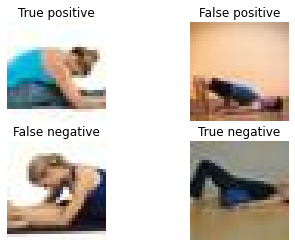
\includegraphics[width=0.7\linewidth]{images/sfb}
	\caption{Example "seatedforwardbend" classifications}
	\label{fig:sfb}
\end{figure}

Conversely, the "mountain" class was the easiest to classify, with only 2 false positives from the "tree" class. This leads more credence to the above theory, where the model seems to be strongly drawing predictions from the overall vertical/horizontal position of the body. Examples of the "mountain" classifications can be seen in figure \ref{fig:mountain}.

\begin{figure}[H]
	\centering
	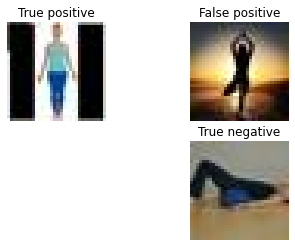
\includegraphics[width=0.7\linewidth]{images/mountain}
	\caption{Example "mountain" classifications}
	\label{fig:mountain}
\end{figure}

\newpage
\section{Visualisation}
The nearest neighbours for two test "bridge" images are shown below in figure \ref{fig:vis_bridge} and figure \ref{fig:vis_bridge_2}.

\begin{figure}[H]
	\centering
	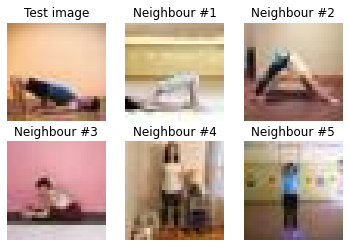
\includegraphics[width=0.7\linewidth]{images/vis_bridge}
	\caption{Nearest neighbours for "bridge" test image}
	\label{fig:vis_bridge}
\end{figure}

\begin{figure}[H]
	\centering
	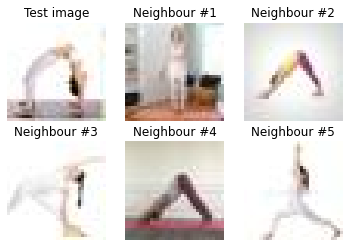
\includegraphics[width=0.7\linewidth]{images/vis_bridge_2}
	\caption{Nearest neighbours for "bridge" test image}
	\label{fig:vis_bridge_2}
\end{figure}

These figures show some limitations of the CNN model - namely, over-reliance on vertical/horizontal position of the body, and inclusion of color as a factor in the predictions (most prevalent in figure \ref{fig:vis_bridge_2}).

The nearest neighbours for a test "tree" image is shown below in figure \ref{fig:vis_tree}. Similarly, the model is overestimating the similarities between images with similar coloured backgrounds. 

\begin{figure}[H]
	\centering
	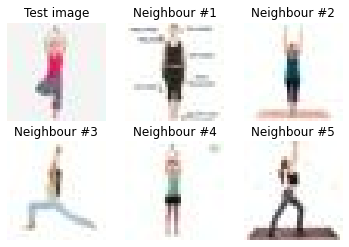
\includegraphics[width=0.7\linewidth]{images/vis_tree}
	\caption{Nearest neighbours for "tree" test image}
	\label{fig:vis_tree}
\end{figure}

A complete visualisation of all test images can be found in the jupyter notebook.

Overall, the CNN model is performing much better than random guesswork, at a accuracy of 54\% compared to an estimated 10\% accuracy when guessing amongst 10 classes. However, as seen above, it is clearly overvaluing non-pose features such as background colours and body size relative to image. It is also not sufficiently separating poses with similar vertical/horizontal components, suggesting a lack of features focusing on limb placement. Likely an edge-detection layer would be beneficial to this CNN to strip out color biases and strengthen limb detection features.

\end{document}

